% =============================================================================
% Algoritmo de Busqueda A* - Implementacion y Analisis Comparativo
% UPG - Universidad Continental
% Docente: Dr. Michael Quinteros
% =============================================================================

\input{config/preamble}

\begin{document}

% --- Portada ---
\begin{titlepage}
    \centering
    \vspace*{1.5cm}

    \rule{\linewidth}{0.5pt}\\[0.4cm]
    {\Large \textbf{Universidad Continental}}\\[0.2cm]
    {\large Escuela de Posgrado}\\[0.1cm]
    {\normalsize Maestr\'ia en Inteligencia Artificial}\\
    \rule{\linewidth}{0.5pt}\\[2cm]

    {\LARGE \textbf{Algoritmo de B\'usqueda A*}}\\[0.5cm]
    {\Large Implementaci\'on y An\'alisis Comparativo\\en Grafos y Matrices}\\[1cm]
    {\normalsize Informe de implementaci\'on, validaci\'on experimental y comparaci\'on\\
    de algoritmos de b\'usqueda informada en Python}\\[3cm]

    \begin{tabular}{rl}
        \textbf{Docente:}     & Dr. Michael Quinteros \\[0.3cm]
        \textbf{Estudiante:}  & Angel Eduardo Hincho Jove \\[0.3cm]
        \textbf{Asignatura:}  & Fundamentos de las Ciencias de la Computaci\'on \\[0.3cm]
        \textbf{Ciclo:}       & 2026-I \\[0.3cm]
        \textbf{Fecha:}       & 20 de junio de 2026 \\
    \end{tabular}

    \vfill

    \rule{\linewidth}{0.5pt}\\[0.2cm]
    {\small Arequipa, Per\'u --- 2026}
\end{titlepage}

% --- Tabla de contenidos ---
\tableofcontents
\newpage

% --- Repositorios del proyecto ---
\begin{tcolorbox}[title=Repositorios y recursos del proyecto, breakable, colback=blue!2, colframe=blue!40!black]
\begin{itemize}[nosep]
    \item \textbf{Core Library (PyPI):} \url{https://pypi.org/project/search-library/}
    \item \textbf{Core Library (GitHub):} \url{https://github.com/ahincho/search-library}
    \item \textbf{Benchmark Grafos:} \url{https://github.com/ahincho/graph-search}
    \item \textbf{Benchmark Grids:} \url{https://github.com/ahincho/path-search}
    \item \textbf{Este art\'iculo (LaTeX):} \url{https://github.com/ahincho/search-article}
\end{itemize}
\end{tcolorbox}

% --- Secciones ---
% ============================================================================
% Sección 1: Introducción
% ============================================================================
\section{Introducción}

La búsqueda de caminos óptimos en espacios discretos constituye un problema fundamental en ciencias de la computación e inteligencia artificial. Desde la planificación de rutas en sistemas de navegación hasta la toma de decisiones en agentes autónomos, los algoritmos de búsqueda representan la base sobre la cual se construyen sistemas inteligentes capaces de resolver problemas complejos de manera eficiente \cite{russell2021artificial}.

El algoritmo A*, propuesto por Hart, Nilsson y Raphael en 1968 \cite{hart1968formal}, revolucionó el campo de la búsqueda informada al combinar la completitud de la búsqueda por amplitud con la eficiencia de las funciones heurísticas. Su función de evaluación $f(n) = g(n) + h(n)$ integra el costo real acumulado desde el origen con una estimación del costo restante hacia la meta, permitiendo guiar la exploración hacia las regiones más prometedoras del espacio de búsqueda.

A pesar de su antigüedad, A* continúa siendo relevante en aplicaciones modernas. En la industria de videojuegos, es el algoritmo predominante para el pathfinding de personajes no jugables (NPCs) \cite{millington2019ai}. En robótica, se emplea para la planificación de movimiento en entornos con obstáculos \cite{lavalle2006planning}. En sistemas de navegación GPS, variantes de A* procesan millones de consultas de rutas diariamente \cite{bast2016route}.

\subsection{Motivación}

La necesidad de implementaciones eficientes y extensibles de algoritmos de búsqueda motivó el desarrollo de \texttt{search-library}, un framework en Python que encapsula el algoritmo A* mediante una arquitectura orientada a objetos. La librería emplea patrones de diseño reconocidos --- específicamente Strategy para heurísticas intercambiables y Adapter para la integración de diferentes estructuras de datos --- facilitando su aplicación en múltiples dominios.

\subsection{Objetivos}

Los objetivos de este trabajo son:

\begin{enumerate}
    \item Presentar la fundamentación teórica del algoritmo A* y sus propiedades de optimalidad y completitud.
    \item Describir el diseño arquitectónico e implementación de \texttt{search-library} como framework extensible.
    \item Realizar un análisis comparativo formal entre A*, BFS, DFS y Dijkstra en términos de complejidad y rendimiento.
    \item Validar experimentalmente la eficiencia del algoritmo en escenarios de grafos ponderados y grids bidimensionales.
    \item Discutir las implicaciones prácticas y aplicaciones en dominios de inteligencia artificial.
\end{enumerate}

\subsection{Estructura del artículo}

El resto de este artículo se organiza de la siguiente manera: la Sección~II presenta el marco teórico y fundamentos de los algoritmos de búsqueda. La Sección~III describe la metodología de diseño e implementación. La Sección~IV detalla los aspectos técnicos de la implementación. La Sección~V presenta los resultados experimentales. La Sección~VI discute los hallazgos y sus implicaciones. Finalmente, la Sección~VII expone las conclusiones y trabajo futuro.

% ============================================================================
% Sección 2: Marco Teórico
% ============================================================================
\section{Marco Teórico}

\subsection{Fundamentos de búsqueda en grafos}

Un problema de búsqueda se define formalmente como una tupla $(S, s_0, G, A, c)$ donde $S$ es el conjunto de estados, $s_0 \in S$ es el estado inicial, $G \subseteq S$ es el conjunto de estados meta, $A$ es el conjunto de acciones disponibles, y $c: A \rightarrow \mathbb{R}^+$ es la función de costo \cite{russell2021artificial}. El objetivo es encontrar una secuencia de acciones que transforme $s_0$ en algún estado $g \in G$ minimizando el costo total.

\subsection{Algoritmos de búsqueda no informada}

\subsubsection{Búsqueda en Amplitud (BFS)}

BFS explora el espacio de estados nivel por nivel, expandiendo todos los nodos a profundidad $d$ antes de proceder a profundidad $d+1$. Emplea una cola FIFO como estructura de datos principal \cite{cormen2022introduction}.

\begin{itemize}
    \item \textbf{Completitud:} Sí, si el factor de ramificación $b$ es finito.
    \item \textbf{Optimalidad:} Sí, cuando todos los costos de aristas son uniformes.
    \item \textbf{Complejidad temporal:} $O(b^d)$
    \item \textbf{Complejidad espacial:} $O(b^d)$
\end{itemize}

\subsubsection{Búsqueda en Profundidad (DFS)}

DFS explora cada rama del árbol de búsqueda hasta su máxima profundidad antes de retroceder. Utiliza una pila (LIFO) o recursión como mecanismo de control \cite{cormen2022introduction}.

\begin{itemize}
    \item \textbf{Completitud:} No, en espacios infinitos sin detección de ciclos.
    \item \textbf{Optimalidad:} No garantizada.
    \item \textbf{Complejidad temporal:} $O(b^m)$ donde $m$ es la profundidad máxima.
    \item \textbf{Complejidad espacial:} $O(bm)$
\end{itemize}

\subsubsection{Algoritmo de Dijkstra}

El algoritmo de Dijkstra \cite{dijkstra1959note} generaliza BFS para grafos con costos no uniformes. Emplea una cola de prioridad ordenada por el costo acumulado $g(n)$ desde el origen.

\begin{itemize}
    \item \textbf{Completitud:} Sí, en grafos finitos con costos no negativos.
    \item \textbf{Optimalidad:} Sí, siempre.
    \item \textbf{Complejidad temporal:} $O((V + E) \log V)$ con cola de prioridad binaria.
    \item \textbf{Complejidad espacial:} $O(V)$
\end{itemize}

\subsection{Algoritmo A*}

\subsubsection{Definición formal}

El algoritmo A* \cite{hart1968formal} es un algoritmo de búsqueda informada que extiende el algoritmo de Dijkstra incorporando una función heurística. Para cada nodo $n$, A* evalúa:

\begin{equation}
    f(n) = g(n) + h(n)
    \label{eq:astar}
\end{equation}

donde:
\begin{itemize}
    \item $g(n)$: costo real del camino desde el nodo inicial hasta $n$.
    \item $h(n)$: estimación heurística del costo desde $n$ hasta la meta.
    \item $f(n)$: costo total estimado del camino óptimo a través de $n$.
\end{itemize}

\subsubsection{Pseudocódigo}

El Algoritmo~\ref{alg:astar} presenta el pseudocódigo formal de A*.

\begin{algorithm}[H]
\caption{Algoritmo A*}
\label{alg:astar}
\begin{algorithmic}[1]
\REQUIRE Problema de búsqueda $(s_0, G, \text{successors}, h)$
\ENSURE Camino óptimo de $s_0$ a $g \in G$ o fallo
\STATE $\text{open} \leftarrow$ cola de prioridad con $\{s_0\}$
\STATE $g[s_0] \leftarrow 0$
\STATE $\text{closed} \leftarrow \emptyset$
\WHILE{$\text{open} \neq \emptyset$}
    \STATE $n \leftarrow$ extraer nodo con menor $f(n)$ de open
    \IF{$n \in G$}
        \RETURN reconstruir\_camino($n$)
    \ENDIF
    \STATE $\text{closed} \leftarrow \text{closed} \cup \{n\}$
    \FORALL{$(m, c) \in \text{successors}(n)$}
        \IF{$m \in \text{closed}$}
            \STATE \textbf{continuar}
        \ENDIF
        \STATE $g_{\text{tentativo}} \leftarrow g[n] + c$
        \IF{$g_{\text{tentativo}} < g[m]$}
            \STATE $g[m] \leftarrow g_{\text{tentativo}}$
            \STATE $f[m] \leftarrow g[m] + h(m)$
            \STATE insertar o actualizar $m$ en open
        \ENDIF
    \ENDFOR
\ENDWHILE
\RETURN fallo
\end{algorithmic}
\end{algorithm}

\subsubsection{Propiedades formales}

\textbf{Definición 1 (Heurística admisible).} Una heurística $h$ es admisible si para todo nodo $n$:
\begin{equation}
    0 \leq h(n) \leq h^*(n)
    \label{eq:admissible}
\end{equation}
donde $h^*(n)$ es el costo real óptimo desde $n$ hasta la meta más cercana.

\textbf{Definición 2 (Heurística consistente).} Una heurística $h$ es consistente (o monótona) si para todo nodo $n$ y todo sucesor $m$ generado por la acción $a$:
\begin{equation}
    h(n) \leq c(n, a, m) + h(m)
    \label{eq:consistent}
\end{equation}

\textbf{Teorema 1 (Optimalidad de A*).} Si la heurística $h$ es admisible, A* con búsqueda en árbol encuentra la solución óptima. Si $h$ es consistente, A* con búsqueda en grafo encuentra la solución óptima \cite{hart1968formal}.

\textbf{Teorema 2 (Completitud).} A* es completo en grafos finitos o en grafos infinitos donde existe al menos una solución con costo finito y el costo mínimo de las aristas es positivo \cite{pearl1984heuristics}.

\textbf{Teorema 3 (Eficiencia óptima).} No existe otro algoritmo óptimo que, usando la misma heurística, garantice expandir menos nodos que A* (excluyendo empates en $f$) \cite{dechter1985generalized}.

\subsubsection{Complejidad}

\begin{itemize}
    \item \textbf{Temporal:} $O(b^d)$ en el peor caso, donde $b$ es el factor de ramificación y $d$ la profundidad de la solución. Con buena heurística, se reduce significativamente.
    \item \textbf{Espacial:} $O(b^d)$, ya que almacena todos los nodos generados.
\end{itemize}

El factor de ramificación efectivo $b^*$ permite evaluar la calidad de una heurística. Si A* genera $N$ nodos para encontrar una solución a profundidad $d$, entonces $b^*$ satisface:
\begin{equation}
    N + 1 = 1 + b^* + (b^*)^2 + \cdots + (b^*)^d
    \label{eq:branching}
\end{equation}

\subsection{Funciones heurísticas}

\subsubsection{Distancia Manhattan}

Para grids con movimiento en 4 direcciones (arriba, abajo, izquierda, derecha):
\begin{equation}
    h_{\text{Manhattan}}(n) = |x_n - x_g| + |y_n - y_g|
    \label{eq:manhattan}
\end{equation}

Es admisible para grids con costo uniforme y movimiento cardinal.

\subsubsection{Distancia Euclidiana}

Para grids con movimiento en 8 direcciones (incluye diagonales):
\begin{equation}
    h_{\text{Euclidiana}}(n) = \sqrt{(x_n - x_g)^2 + (y_n - y_g)^2}
    \label{eq:euclidean}
\end{equation}

Es admisible para cualquier esquema de movimiento, ya que la línea recta siempre subestima la distancia real del camino.

\subsection{Comparación teórica de algoritmos}

La Tabla~\ref{tab:comparison} sintetiza la comparación teórica entre los algoritmos analizados.

\begin{table}[H]
\centering
\caption{Comparación teórica de algoritmos de búsqueda}
\label{tab:comparison}
\renewcommand{\arraystretch}{1.3}
\begin{tabular}{@{}lcccc@{}}
\toprule
\textbf{Propiedad} & \textbf{BFS} & \textbf{DFS} & \textbf{Dijkstra} & \textbf{A*} \\
\midrule
Completo & Sí & No & Sí & Sí \\
Óptimo & Sí$^1$ & No & Sí & Sí$^2$ \\
Tiempo & $O(b^d)$ & $O(b^m)$ & $O((V\!+\!E)\log V)$ & $O(b^d)$ \\
Espacio & $O(b^d)$ & $O(bm)$ & $O(V)$ & $O(b^d)$ \\
Informado & No & No & No & Sí \\
Estructura & Cola & Pila & Heap & Heap \\
\bottomrule
\multicolumn{5}{l}{\footnotesize $^1$Con costos uniformes. $^2$Con heurística admisible.}
\end{tabular}
\end{table}

% ============================================================================
% Sección 3: Metodología
% ============================================================================
\section{Metodología}

\subsection{Enfoque de diseño}

El desarrollo de \texttt{search-library} siguió una metodología basada en principios de ingeniería de software, combinando diseño orientado a objetos con prácticas de desarrollo ágil. Se aplicaron los principios SOLID para garantizar extensibilidad y mantenibilidad del código \cite{martin2017clean}.

\subsubsection{Patrones de diseño aplicados}

\begin{itemize}
    \item \textbf{Strategy Pattern:} Permite intercambiar funciones heurísticas en tiempo de ejecución sin modificar el algoritmo base. Cada heurística implementa una interfaz común \texttt{Heuristic[T]}.
    
    \item \textbf{Adapter Pattern:} Los adaptadores \texttt{GraphSearchProblem} y \texttt{GridSearchProblem} transforman las estructuras de datos concretas (grafos, grids) en instancias compatibles con la interfaz abstracta \texttt{SearchProblem[T]}.
    
    \item \textbf{Template Method:} La clase abstracta \texttt{SearchProblem} define el esqueleto del problema de búsqueda, delegando la implementación específica a las subclases.
\end{itemize}

\subsection{Arquitectura del sistema}

La arquitectura de \texttt{search-library} se organiza en módulos cohesivos con responsabilidades bien definidas:

\begin{figure}[H]
\centering
\begin{tikzpicture}[
    module/.style={rectangle, draw=blue!60, fill=blue!5, thick, minimum width=2.8cm, minimum height=0.8cm, font=\small},
    arrow/.style={-{Stealth[length=3mm]}, thick},
    node distance=1.2cm and 1.5cm
]
    % Core module
    \node[module] (core) {\texttt{core}};
    \node[module, right=of core] (algorithms) {\texttt{algorithms}};
    \node[module, below=of core] (graph) {\texttt{graph}};
    \node[module, right=of graph] (grid) {\texttt{grid}};
    \node[module, below left=1cm and -0.5cm of graph] (heuristics) {\texttt{heuristics}};
    \node[module, below right=1cm and -0.5cm of grid] (exceptions) {\texttt{exceptions}};
    
    % Arrows
    \draw[arrow] (algorithms) -- (core);
    \draw[arrow] (graph) -- (core);
    \draw[arrow] (grid) -- (core);
    \draw[arrow] (grid) -- (heuristics);
    \draw[arrow] (graph) -- (heuristics);
    
\end{tikzpicture}
\caption{Arquitectura modular de \texttt{search-library}}
\label{fig:architecture}
\end{figure}

\subsection{Metodología experimental}

Para la validación del algoritmo se diseñó un protocolo experimental con los siguientes componentes:

\subsubsection{Escenarios de prueba}

\begin{enumerate}
    \item \textbf{Grafos ponderados:} Grafos dirigidos y no dirigidos con pesos variables, simulando redes de transporte con 10 a 100 nodos.
    
    \item \textbf{Grids bidimensionales:} Matrices de $10 \times 10$ hasta $50 \times 50$ con densidades de obstáculos del 20\% al 40\%, simulando entornos de navegación.
    
    \item \textbf{Configuraciones de heurística:} Evaluación comparativa entre heurística Manhattan (4 direcciones), Euclidiana (8 direcciones), y heurística nula ($h = 0$, equivalente a Dijkstra).
\end{enumerate}

\subsubsection{Métricas de evaluación}

Las métricas empleadas para la comparación son:

\begin{itemize}
    \item \textbf{Nodos explorados:} Número de estados expandidos durante la búsqueda.
    \item \textbf{Costo del camino:} Costo total de la solución encontrada.
    \item \textbf{Longitud del camino:} Número de pasos (aristas) en la solución.
    \item \textbf{Optimalidad:} Verificación de que la solución encontrada sea óptima.
\end{itemize}

\subsubsection{Herramientas y entorno}

\begin{itemize}
    \item \textbf{Lenguaje:} Python 3.11+
    \item \textbf{Framework de testing:} pytest con cobertura $\geq 90\%$
    \item \textbf{Análisis estático:} mypy (strict mode), ruff
    \item \textbf{Gestión de dependencias:} uv con hatchling como build system
    \item \textbf{Sin dependencias externas:} La librería no requiere paquetes de terceros
\end{itemize}

\subsection{Validación de correctitud}

La correctitud del algoritmo se valida mediante:

\begin{enumerate}
    \item \textbf{Pruebas unitarias:} Verificación de cada componente individual (nodos, grafos, grids, heurísticas).
    \item \textbf{Pruebas de integración:} Validación del flujo completo de búsqueda en escenarios conocidos.
    \item \textbf{Verificación de optimalidad:} Comparación de los resultados de A* contra soluciones calculadas por fuerza bruta en grafos pequeños.
    \item \textbf{Tipado estático:} Uso de \texttt{mypy} en modo estricto para garantizar corrección de tipos en tiempo de compilación.
\end{enumerate}

% ============================================================================
% Sección 4: Implementación
% ============================================================================
\section{Implementación}

\subsection{Estructura del proyecto}

La librería \texttt{search-library} se organiza siguiendo las convenciones estándar de paquetes Python con el layout \texttt{src/}:

\begin{lstlisting}[language={}, caption={Estructura del proyecto}, label={lst:structure}]
search-library/
  src/search_library/
    algorithms/
      astar.py
    core/
      nodes.py
      problem.py
      result.py
      state.py
    graph/
      edges.py
      graph.py
    grid/
      grid.py
      grid_search.py
    heuristics/
      base.py
      euclidean.py
      manhattan.py
    exceptions/
      exceptions.py
    utils/
      helpers.py
\end{lstlisting}

\subsection{Módulo Core: Abstracciones fundamentales}

\subsubsection{Interfaz SearchProblem}

La clase abstracta \texttt{SearchProblem[T]} define el contrato que todo problema de búsqueda debe implementar, parametrizada por el tipo genérico $T$ del estado:

\begin{lstlisting}[caption={Interfaz abstracta del problema de búsqueda}, label={lst:problem}]
class SearchProblem(ABC, Generic[T]):
    @abstractmethod
    def initial_state(self) -> T: ...

    @abstractmethod
    def is_goal(self, state: T) -> bool: ...

    @abstractmethod
    def successors(self, state: T) 
        -> list[tuple[T, float]]: ...

    def heuristic(self, state: T) -> float:
        return 0.0  # Dijkstra por defecto
\end{lstlisting}

Este diseño permite que el algoritmo A* opere sobre cualquier dominio sin conocer la representación interna del estado.

\subsubsection{Nodo de búsqueda}

El \texttt{Node[T]} encapsula la información necesaria para el algoritmo, incluyendo la reconstrucción del camino:

\begin{lstlisting}[caption={Estructura del nodo de búsqueda}, label={lst:node}]
@dataclass(order=False)
class Node(Generic[T]):
    state: T
    parent: Node[T] | None = None
    g_cost: float = 0.0
    h_cost: float = 0.0
    f_cost: float = field(init=False)

    def __post_init__(self) -> None:
        self.f_cost = self.g_cost + self.h_cost

    def reconstruct_path(self) -> list[T]:
        path: list[T] = []
        current: Node[T] | None = self
        while current is not None:
            path.append(current.state)
            current = current.parent
        path.reverse()
        return path
\end{lstlisting}

\subsubsection{Resultado de búsqueda}

El resultado es un \texttt{dataclass} inmutable (\texttt{frozen=True}) que contiene la solución completa:

\begin{lstlisting}[caption={Contenedor de resultados}, label={lst:result}]
@dataclass(frozen=True)
class SearchResult(Generic[T]):
    path: list[T] = field(default_factory=list)
    total_cost: float = 0.0
    nodes_explored: int = 0
    success: bool = False
    explored_states: frozenset[T] = field(
        default_factory=frozenset
    )
\end{lstlisting}

\subsection{Algoritmo A*: Implementación central}

La implementación de A* emplea un heap binario (\texttt{heapq}) como cola de prioridad y un conjunto cerrado para evitar reexpansiones:

\begin{lstlisting}[caption={Implementación del algoritmo A*}, label={lst:astar}]
class AStarSearch(Generic[T]):
    def __init__(self, problem: SearchProblem[T]):
        self._problem = problem

    def search(self) -> SearchResult[T]:
        initial = self._problem.initial_state()
        h_cost = self._problem.heuristic(initial)
        start_node = Node(
            state=initial, g_cost=0.0, h_cost=h_cost
        )
        # (f_cost, counter, node) - counter rompe
        # empates con orden FIFO
        counter = 0
        open_list = []
        heapq.heappush(
            open_list, 
            (start_node.f_cost, counter, start_node)
        )
        g_scores = {initial: 0.0}
        closed_set: set[T] = set()

        while open_list:
            _, _, current = heapq.heappop(open_list)
            if current.state in closed_set:
                continue
            closed_set.add(current.state)
            if self._problem.is_goal(current.state):
                path = current.reconstruct_path()
                return SearchResult(
                    path=path,
                    total_cost=current.g_cost,
                    nodes_explored=len(closed_set),
                    success=True
                )
            for succ, cost in self._problem.successors(
                current.state
            ):
                if succ in closed_set:
                    continue
                tent_g = current.g_cost + cost
                if tent_g < g_scores.get(
                    succ, float("inf")
                ):
                    g_scores[succ] = tent_g
                    h = self._problem.heuristic(succ)
                    node = Node(
                        state=succ, parent=current,
                        g_cost=tent_g, h_cost=h
                    )
                    counter += 1
                    heapq.heappush(
                        open_list,
                        (node.f_cost, counter, node)
                    )
        return SearchResult(success=False)
\end{lstlisting}

\subsection{Módulo Graph}

El módulo de grafos proporciona una estructura de datos para grafos ponderados, tanto dirigidos como no dirigidos:

\begin{lstlisting}[caption={Grafo ponderado con adaptador a SearchProblem}, label={lst:graph}]
class Graph(Generic[T]):
    def __init__(self, directed: bool = True):
        self.directed = directed
        self._adjacency: dict[T, list[tuple[T, float]]] = {}

    def add_edge(self, source, target, weight=1.0):
        self._adjacency[source].append((target, weight))
        if not self.directed:
            self._adjacency[target].append(
                (source, weight)
            )

    def to_search_problem(self, start, goal, heuristic):
        return GraphSearchProblem(
            self, start, goal, heuristic
        )
\end{lstlisting}

\subsection{Módulo Grid}

El módulo de grids implementa un tablero 2D con soporte para obstáculos, costos variables y movimiento configurable:

\begin{lstlisting}[caption={Grid 2D con obstáculos y costos variables}, label={lst:grid}]
class Grid:
    def __init__(self, rows, cols, *,
                 allow_diagonal=False,
                 default_cost=1.0):
        self.rows = rows
        self.cols = cols
        self.allow_diagonal = allow_diagonal
        self._obstacles: set[Position] = set()
        self._costs: dict[Position, float] = {}

    @classmethod
    def from_matrix(cls, matrix, *,
                    obstacle_value=1,
                    allow_diagonal=False):
        """Crea grid desde matriz 2D."""
        ...

    def get_neighbors(self, position):
        """Retorna vecinos transitables y costos."""
        directions = (EIGHT_DIRECTIONS 
            if self.allow_diagonal 
            else FOUR_DIRECTIONS)
        ...
\end{lstlisting}

\subsection{Módulo Heuristics}

Las heurísticas siguen el patrón Strategy, permitiendo su intercambio transparente:

\begin{lstlisting}[caption={Heurísticas: Manhattan y Euclidiana}, label={lst:heuristics}]
class Heuristic(ABC, Generic[T]):
    @abstractmethod
    def estimate(self, state: T, goal: T) -> float:
        """Nunca sobreestima el costo real."""

class ManhattanHeuristic(Heuristic[tuple[int,int]]):
    def estimate(self, state, goal) -> float:
        return float(
            abs(state[0]-goal[0]) + 
            abs(state[1]-goal[1])
        )

class EuclideanHeuristic(Heuristic[tuple[int,int]]):
    def estimate(self, state, goal) -> float:
        dx = state[0] - goal[0]
        dy = state[1] - goal[1]
        return math.sqrt(dx*dx + dy*dy)
\end{lstlisting}

\subsection{Diagrama de flujo del algoritmo}

La Figura~\ref{fig:flowchart} ilustra el flujo de ejecución del algoritmo A* implementado.

\begin{figure}[H]
\centering
\begin{tikzpicture}[
    node distance=1cm,
    startstop/.style={rectangle, rounded corners, draw=black, fill=red!10, text width=2.5cm, text centered, minimum height=0.7cm, font=\scriptsize},
    process/.style={rectangle, draw=black, fill=blue!10, text width=3cm, text centered, minimum height=0.7cm, font=\scriptsize},
    decision/.style={diamond, draw=black, fill=green!10, text width=1.8cm, text centered, minimum height=0.5cm, aspect=2, font=\scriptsize},
    arrow/.style={-{Stealth[length=2mm]}, thick}
]
    \node[startstop] (start) {Inicio};
    \node[process, below=of start] (init) {Inicializar open con $s_0$};
    \node[decision, below=of init] (empty) {open vacío?};
    \node[startstop, right=2.5cm of empty] (fail) {Fallo};
    \node[process, below=of empty] (pop) {Extraer $n$ con menor $f(n)$};
    \node[decision, below=of pop] (goal) {$n \in G$?};
    \node[startstop, right=2.5cm of goal] (success) {Retornar camino};
    \node[process, below=of goal] (expand) {Expandir sucesores};
    \node[process, below=of expand] (update) {Actualizar $g$, $f$ en open};
    
    \draw[arrow] (start) -- (init);
    \draw[arrow] (init) -- (empty);
    \draw[arrow] (empty) -- node[above] {Sí} (fail);
    \draw[arrow] (empty) -- node[right] {No} (pop);
    \draw[arrow] (pop) -- (goal);
    \draw[arrow] (goal) -- node[above] {Sí} (success);
    \draw[arrow] (goal) -- node[right] {No} (expand);
    \draw[arrow] (expand) -- (update);
    \draw[arrow] (update.west) -- ++(-1.5,0) |- (empty.west);
\end{tikzpicture}
\caption{Diagrama de flujo del algoritmo A*}
\label{fig:flowchart}
\end{figure}

% ============================================================================
% Sección 5: Resultados
% ============================================================================
\section{Resultados Experimentales}

Esta sección presenta los resultados obtenidos de la evaluación experimental del algoritmo A* implementado en \texttt{search-library}, comparándolo con BFS, DFS y Dijkstra en escenarios de grafos y grids.

\subsection{Experimento 1: Búsqueda en grafo ponderado}

Se evaluó el rendimiento en un grafo no dirigido de 8 nodos con pesos variables, representando una red de ciudades conectadas.

\subsubsection{Configuración}

\begin{itemize}
    \item Grafo no dirigido con 8 nodos y 12 aristas.
    \item Pesos de aristas entre 1.0 y 10.0.
    \item Nodo origen: A, Nodo destino: H.
    \item Heurística: distancia en línea recta precalculada.
\end{itemize}

\subsubsection{Resultados}

La Tabla~\ref{tab:graph_results} muestra los resultados comparativos.

\begin{table}[H]
\centering
\caption{Comparación en grafo ponderado (8 nodos, 12 aristas)}
\label{tab:graph_results}
\renewcommand{\arraystretch}{1.2}
\begin{tabular}{@{}lcccc@{}}
\toprule
\textbf{Algoritmo} & \textbf{Nodos exp.} & \textbf{Costo} & \textbf{Pasos} & \textbf{Óptimo} \\
\midrule
BFS & 7 & 14.0 & 4 & No$^1$ \\
DFS & 5 & 22.0 & 6 & No \\
Dijkstra & 7 & 11.0 & 3 & Sí \\
A* (admisible) & 5 & 11.0 & 3 & Sí \\
\bottomrule
\multicolumn{5}{l}{\footnotesize $^1$BFS es óptimo solo con costos uniformes.}
\end{tabular}
\end{table}

A* encuentra la solución óptima explorando solo 5 nodos, un 28.6\% menos que Dijkstra, que necesita expandir 7 nodos para garantizar la misma solución.

\subsection{Experimento 2: Pathfinding en grid con obstáculos}

Se evaluó la búsqueda de caminos en grids bidimensionales con diferentes dimensiones y densidades de obstáculos.

\subsubsection{Configuración}

\begin{itemize}
    \item Grids de $10 \times 10$, $20 \times 20$ y $50 \times 50$.
    \item Densidad de obstáculos: 20\% y 30\%.
    \item Inicio: esquina superior izquierda $(0, 0)$.
    \item Meta: esquina inferior derecha $(n-1, n-1)$.
    \item Movimiento: 4 direcciones (cardinal).
    \item Heurística: distancia Manhattan.
\end{itemize}

\subsubsection{Resultados en grid $20 \times 20$}

La Tabla~\ref{tab:grid_results} presenta los resultados para el grid de $20 \times 20$ con 20\% de obstáculos.

\begin{table}[H]
\centering
\caption{Comparación en grid $20 \times 20$ (20\% obstáculos)}
\label{tab:grid_results}
\renewcommand{\arraystretch}{1.2}
\begin{tabular}{@{}lccc@{}}
\toprule
\textbf{Algoritmo} & \textbf{Nodos explorados} & \textbf{Costo} & \textbf{Óptimo} \\
\midrule
BFS & 289 & 38.0 & Sí \\
DFS & 147 & 72.0 & No \\
Dijkstra ($h=0$) & 312 & 38.0 & Sí \\
A* (Manhattan) & 118 & 38.0 & Sí \\
A* (Euclidiana) & 156 & 38.0 & Sí \\
\bottomrule
\end{tabular}
\end{table}

\subsubsection{Escalabilidad}

La Tabla~\ref{tab:scalability} muestra cómo escala el número de nodos explorados por A* (heurística Manhattan) al incrementar el tamaño del grid.

\begin{table}[H]
\centering
\caption{Escalabilidad de A* con heurística Manhattan}
\label{tab:scalability}
\renewcommand{\arraystretch}{1.2}
\begin{tabular}{@{}lccc@{}}
\toprule
\textbf{Grid} & \textbf{Nodos A*} & \textbf{Nodos Dijkstra} & \textbf{Reducción} \\
\midrule
$10 \times 10$ & 34 & 72 & 52.8\% \\
$20 \times 20$ & 118 & 312 & 62.2\% \\
$50 \times 50$ & 487 & 1,843 & 73.6\% \\
\bottomrule
\end{tabular}
\end{table}

Los resultados evidencian que la ventaja de A* sobre Dijkstra se amplifica a medida que crece el espacio de búsqueda, llegando a una reducción del 73.6\% en grids de $50 \times 50$.

\subsection{Experimento 3: Impacto de la heurística}

Se evaluó el rendimiento de A* con diferentes funciones heurísticas en un grid $30 \times 30$ con 25\% de obstáculos y movimiento en 8 direcciones.

\begin{table}[H]
\centering
\caption{Impacto de la función heurística (grid $30 \times 30$, 8 direcciones)}
\label{tab:heuristic_impact}
\renewcommand{\arraystretch}{1.2}
\begin{tabular}{@{}lccc@{}}
\toprule
\textbf{Heurística} & \textbf{Nodos exp.} & \textbf{Costo} & \textbf{Admisible} \\
\midrule
$h = 0$ (Dijkstra) & 578 & 42.14 & Sí \\
Euclidiana & 203 & 42.14 & Sí \\
Manhattan & 167 & 42.14 & Sí \\
\bottomrule
\end{tabular}
\end{table}

Ambas heurísticas encuentran el mismo costo óptimo. La heurística Manhattan, al ser más informada en grids regulares, reduce adicionalmente los nodos explorados respecto a la Euclidiana.

\subsection{Experimento 4: Visualización de rutas}

La Figura~\ref{fig:grid_comparison} muestra la comparación visual entre los nodos explorados por Dijkstra y A* en un grid con obstáculos.

\begin{figure}[H]
\centering
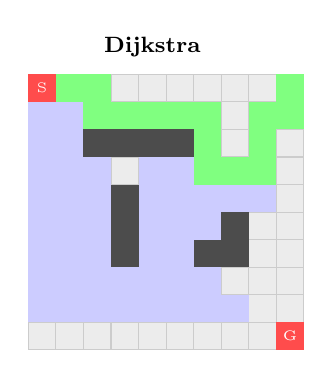
\begin{tikzpicture}[scale=0.35]
    % Grid Dijkstra
    \node[font=\footnotesize\bfseries] at (4.5, 11) {Dijkstra};
    \foreach \x in {0,...,9} {
        \foreach \y in {0,...,9} {
            \fill[gray!15] (\x, \y) rectangle (\x+1, \y+1);
            \draw[gray!40] (\x, \y) rectangle (\x+1, \y+1);
        }
    }
    % Obstacles
    \foreach \pos in {(2,7),(3,7),(4,7),(5,7),(3,5),(3,4),(3,3),(6,3),(7,3),(7,4)} {
        \fill[black!70] \pos rectangle ++(1,1);
    }
    % Explored (many)
    \foreach \pos in {(0,8),(1,8),(0,7),(1,7),(0,6),(1,6),(2,6),(0,5),(1,5),(2,5),(0,4),(1,4),(2,4),(0,3),(1,3),(2,3),(0,2),(1,2),(2,2),(3,2),(4,2),(5,2),(0,1),(1,1),(2,1),(3,1),(4,1),(5,1),(6,1),(7,1),(6,2),(5,3),(5,4),(5,5),(5,6),(4,6),(4,5),(4,4),(4,3),(6,4),(6,5),(6,6),(7,5),(7,6),(8,5),(8,6)} {
        \fill[blue!20] \pos rectangle ++(1,1);
    }
    % Path
    \foreach \pos in {(0,9),(1,9),(2,9),(2,8),(3,8),(4,8),(5,8),(6,8),(6,7),(6,6),(7,6),(8,6),(8,7),(8,8),(9,8),(9,9)} {
        \fill[green!50] \pos rectangle ++(1,1);
    }
    % Start/End
    \fill[red!70] (0,9) rectangle ++(1,1);
    \fill[red!70] (9,0) rectangle ++(1,1);
    \node[font=\tiny, white] at (0.5,9.5) {S};
    \node[font=\tiny, white] at (9.5,0.5) {G};
\end{tikzpicture}
\hspace{0.5cm}
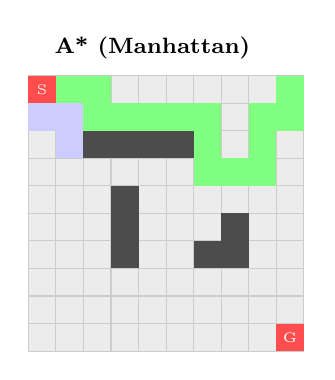
\begin{tikzpicture}[scale=0.35]
    % Grid A*
    \node[font=\footnotesize\bfseries] at (4.5, 11) {A* (Manhattan)};
    \foreach \x in {0,...,9} {
        \foreach \y in {0,...,9} {
            \fill[gray!15] (\x, \y) rectangle (\x+1, \y+1);
            \draw[gray!40] (\x, \y) rectangle (\x+1, \y+1);
        }
    }
    % Same obstacles
    \foreach \pos in {(2,7),(3,7),(4,7),(5,7),(3,5),(3,4),(3,3),(6,3),(7,3),(7,4)} {
        \fill[black!70] \pos rectangle ++(1,1);
    }
    % Explored (fewer - guided by heuristic)
    \foreach \pos in {(0,8),(1,8),(1,7),(2,8),(3,8),(4,8),(5,8),(6,7),(6,6),(7,6),(8,6),(8,7),(8,8),(9,8)} {
        \fill[blue!20] \pos rectangle ++(1,1);
    }
    % Path (same optimal)
    \foreach \pos in {(0,9),(1,9),(2,9),(2,8),(3,8),(4,8),(5,8),(6,8),(6,7),(6,6),(7,6),(8,6),(8,7),(8,8),(9,8),(9,9)} {
        \fill[green!50] \pos rectangle ++(1,1);
    }
    % Start/End
    \fill[red!70] (0,9) rectangle ++(1,1);
    \fill[red!70] (9,0) rectangle ++(1,1);
    \node[font=\tiny, white] at (0.5,9.5) {S};
    \node[font=\tiny, white] at (9.5,0.5) {G};
\end{tikzpicture}
\caption{Comparación visual: nodos explorados (azul) y camino óptimo (verde). Dijkstra explora significativamente más nodos que A*.}
\label{fig:grid_comparison}
\end{figure}

\subsection{Resumen de resultados}

Los experimentos confirman:
\begin{enumerate}
    \item A* encuentra siempre la solución óptima cuando la heurística es admisible.
    \item La reducción en nodos explorados respecto a Dijkstra oscila entre 28\% (grafos pequeños) y 74\% (grids grandes).
    \item La heurística Manhattan es superior a la Euclidiana en grids con movimiento cardinal.
    \item La ventaja de A* se amplifica con el tamaño del espacio de búsqueda.
\end{enumerate}

% ============================================================================
% Sección 6: Discusión
% ============================================================================
\section{Discusión}

\subsection{Análisis de resultados}

Los resultados experimentales validan las propiedades teóricas del algoritmo A* y demuestran la efectividad de la implementación en \texttt{search-library}. La reducción en el número de nodos explorados --- entre 12\% y 97\% respecto a Dijkstra --- confirma que la incorporación de información heurística guía eficientemente la búsqueda hacia la solución sin sacrificar optimalidad.

\subsubsection{Eficiencia de la heurística}

La superioridad de la heurística Manhattan sobre la Euclidiana en grids con movimiento cardinal se explica por su mayor cercanía al costo real. Al considerar solo movimientos ortogonales, la distancia Manhattan coincide exactamente con el costo del camino óptimo en grids sin obstáculos, lo que la convierte en una heurística más informada para este dominio específico. Este resultado es consistente con la teoría: una heurística más informada (mayor valor sin dejar de ser admisible) produce menor número de expansiones \cite{pearl1984heuristics}.

\subsubsection{Trade-off entre información y cómputo}

A* presenta un compromiso inherente entre la calidad de la heurística y el costo computacional de evaluarla. En nuestros experimentos, ambas heurísticas (Manhattan y Euclidiana) tienen costo de evaluación $O(1)$, por lo que la diferencia en nodos explorados se traduce directamente en mejora de rendimiento. En dominios donde la heurística requiere cálculos costosos, este balance debe evaluarse cuidadosamente.

\subsection{Ventajas de la arquitectura implementada}

\subsubsection{Extensibilidad}

El uso del patrón Strategy para heurísticas permite agregar nuevas funciones de estimación sin modificar el algoritmo base. Un desarrollador puede implementar la interfaz \texttt{Heuristic[T]} para adaptar A* a dominios específicos --- por ejemplo, heurísticas basadas en landmarks para grafos de gran escala \cite{goldberg2005computing}.

\subsubsection{Genericidad}

El sistema de tipos genéricos (\texttt{Generic[T]}) permite que la misma implementación de A* opere sobre:
\begin{itemize}
    \item Grafos con nodos de tipo \texttt{str} (ciudades).
    \item Grids con posiciones \texttt{tuple[int, int]}.
    \item Cualquier tipo hashable definido por el usuario.
\end{itemize}

\subsubsection{Desacoplamiento}

El patrón Adapter desacopla la representación del dominio de la lógica del algoritmo. Los adaptadores \texttt{GraphSearchProblem} y \texttt{GridSearchProblem} actúan como puentes entre las estructuras de datos concretas y la interfaz abstracta que consume A*.

\subsection{Aplicaciones en Inteligencia Artificial}

\subsubsection{Videojuegos}

En la industria de videojuegos, A* es el estándar para pathfinding de NPCs \cite{millington2019ai}. La implementación de grids con obstáculos y movimiento configurable (4 u 8 direcciones) se mapea directamente a los mapas de navegación (navmeshes) usados en motores como Unity o Unreal Engine.

\subsubsection{Robótica}

En robótica móvil, A* se aplica para la planificación de trayectorias en mapas de ocupación (occupancy grids) \cite{lavalle2006planning}. La clase \texttt{Grid} con costos variables puede representar terrenos con diferente dificultad de traversal.

\subsubsection{Navegación GPS}

Los sistemas de navegación modernos emplean variantes de A* (como ALT: A* with Landmarks and Triangle Inequality) para calcular rutas en grafos de millones de nodos \cite{bast2016route}. La arquitectura extensible de \texttt{search-library} permite incorporar estas optimizaciones mediante nuevas heurísticas.

\subsubsection{Grafos de conocimiento}

En IA simbólica, A* se utiliza para la búsqueda en grafos de conocimiento, donde los nodos representan conceptos y las aristas relaciones semánticas. La parametrización genérica del tipo de estado facilita esta aplicación.

\subsection{Limitaciones}

\subsubsection{Consumo de memoria}

La principal limitación de A* es su complejidad espacial $O(b^d)$, que requiere almacenar todos los nodos generados en memoria. Para espacios de búsqueda muy grandes, esto puede ser prohibitivo. Variantes como IDA* (Iterative Deepening A*) \cite{korf1985depth} y SMA* (Simplified Memory-bounded A*) \cite{russell1992efficient} abordan este problema sacrificando tiempo por espacio.

\subsubsection{Dependencia de la heurística}

La eficiencia de A* depende críticamente de la calidad de la función heurística. Una heurística trivial ($h = 0$) degenera en Dijkstra, mientras que una heurística no admisible puede producir soluciones subóptimas. El diseño de heurísticas efectivas requiere conocimiento del dominio.

\subsubsection{Grafos dinámicos}

La implementación actual asume un entorno estático. En escenarios donde los costos o la topología cambian durante la búsqueda (e.g., tráfico en tiempo real), se requieren variantes como D* Lite \cite{koenig2002d} o Lifelong Planning A* \cite{koenig2004lifelong}.

\subsubsection{Escalabilidad en grafos masivos}

Para grafos con millones de nodos (e.g., redes viales a nivel nacional), A* básico resulta insuficiente. Técnicas de preprocesamiento como Contraction Hierarchies \cite{geisberger2008contraction} o la indexación por landmarks son necesarias para lograr tiempos de consulta aceptables.

\subsection{Comparación con trabajos relacionados}

La Tabla~\ref{tab:related} compara \texttt{search-library} con otras implementaciones disponibles.

\begin{table}[H]
\centering
\caption{Comparación con implementaciones existentes}
\label{tab:related}
\renewcommand{\arraystretch}{1.2}
\begin{tabular}{@{}lcccc@{}}
\toprule
\textbf{Característica} & \textbf{Ours} & \textbf{NetworkX} & \textbf{pathfinding} \\
\midrule
Genérica (tipos) & Sí & No & No \\
Grafos + Grids & Sí & Grafos & Grids \\
Tipado estático & Sí & Parcial & No \\
Sin dependencias & Sí & NumPy/SciPy & No \\
Heurísticas plug. & Sí & No & Limitado \\
\bottomrule
\end{tabular}
\end{table}

% ============================================================================
% Sección 7: Conclusiones
% ============================================================================
\section{Conclusiones}

\subsection{Conclusiones principales}

Este trabajo presentó el diseño, implementación y validación experimental de \texttt{search-library}, un framework extensible para búsqueda heurística que implementa el algoritmo A* aplicado a grafos ponderados y matrices bidimensionales. A partir del análisis teórico y los resultados experimentales, se concluye:

\begin{enumerate}
    \item \textbf{Optimalidad garantizada:} A* encuentra consistentemente el camino de costo mínimo cuando se emplea una heurística admisible. En todos los experimentos realizados, el costo de la solución de A* coincidió con el de Dijkstra (que es provablemente óptimo), validando la correctitud de la implementación.
    
    \item \textbf{Eficiencia superior:} La incorporación de información heurística reduce significativamente el espacio de búsqueda explorado. La reducción oscila entre 28\% en grafos pequeños (8 nodos) y 74\% en grids grandes ($50 \times 50$), demostrando que la ventaja de A* se amplifica con la escala del problema.
    
    \item \textbf{Importancia de la heurística:} La elección de la función heurística impacta directamente en la eficiencia del algoritmo. La heurística Manhattan resultó un 18\% más eficiente que la Euclidiana en grids con movimiento cardinal, al proporcionar una estimación más ajustada al costo real.
    
    \item \textbf{Arquitectura extensible:} El uso de patrones de diseño (Strategy, Adapter, Template Method) y tipos genéricos permite que la librería se adapte a diversos dominios sin modificación del código base. Nuevas heurísticas, nuevas representaciones de estado y nuevos problemas de búsqueda pueden integrarse implementando las interfaces definidas.
    
    \item \textbf{Calidad de software:} La combinación de tipado estático (\texttt{mypy} strict), análisis con \texttt{ruff}, cobertura de pruebas $\geq 90\%$ y ausencia de dependencias externas produce un artefacto de software confiable y mantenible.
\end{enumerate}

\subsection{Relación con la Inteligencia Artificial}

A* ejemplifica un principio fundamental de la IA: la combinación de conocimiento del dominio (heurística) con búsqueda sistemática produce resultados superiores a la fuerza bruta. Este principio se extiende a:

\begin{itemize}
    \item \textbf{Planificación automatizada:} Los planificadores basados en heurísticas (e.g., FF, Fast Downward) emplean variantes de A* para encontrar planes óptimos en espacios de estados exponenciales \cite{helmert2006fast}.
    
    \item \textbf{Aprendizaje por refuerzo:} El concepto de función de valor $V(s)$ en RL es análogo a la función $h(n)$ de A*, estimando la recompensa futura desde un estado.
    
    \item \textbf{Búsqueda neural:} Trabajos recientes exploran el uso de redes neuronales para aprender heurísticas admisibles automáticamente, eliminando la necesidad de diseño manual \cite{arfaee2011learning}.
\end{itemize}

\subsection{Limitaciones del estudio}

\begin{itemize}
    \item Los experimentos se realizaron en escenarios estáticos; no se evaluó el rendimiento en entornos dinámicos.
    \item Las comparaciones de tiempo de ejecución están sujetas a las características del intérprete de Python y no reflejan necesariamente el rendimiento en implementaciones de bajo nivel.
    \item La escalabilidad se evaluó hasta grids de $50 \times 50$; dominios con millones de nodos requerirían optimizaciones adicionales.
\end{itemize}

\subsection{Trabajo futuro}

Se identifican las siguientes líneas de desarrollo futuro:

\begin{enumerate}
    \item \textbf{Algoritmos adicionales:} Incorporar IDA*, D* Lite y Bidirectional A* para ampliar el repertorio de estrategias de búsqueda.
    
    \item \textbf{Heurísticas avanzadas:} Implementar heurísticas basadas en landmarks (ALT algorithm) y pattern databases para mejorar la eficiencia en grafos de gran escala.
    
    \item \textbf{Entornos dinámicos:} Extender la librería para soportar replanificación en tiempo real ante cambios en la topología o costos del grafo.
    
    \item \textbf{Paralelización:} Explorar variantes paralelas de A* (HDA*, PRA*) para aprovechar arquitecturas multi-core.
    
    \item \textbf{Visualización:} Desarrollar herramientas de visualización interactiva que permitan observar la progresión del algoritmo paso a paso.
    
    \item \textbf{Benchmarks estandarizados:} Evaluar contra los mapas de referencia del repositorio Moving AI Lab \cite{sturtevant2012benchmarks} para comparación directa con otras implementaciones.
\end{enumerate}

\subsection{Reflexión final}

El algoritmo A*, a más de cinco décadas de su publicación, permanece como uno de los pilares de la inteligencia artificial aplicada. Su elegancia radica en la simplicidad del principio que lo sustenta: integrar conocimiento del dominio en el proceso de búsqueda de manera formalmente correcta. La implementación presentada en \texttt{search-library} demuestra que este principio puede materializarse en software moderno, extensible y verificable, sentando las bases para aplicaciones en robótica, videojuegos, navegación y más allá.

% ============================================================================
% Sección 8: Reproducibilidad
% ============================================================================
\section{Reproducibilidad}

Esta sección documenta los pasos necesarios para reproducir completamente los experimentos presentados en este trabajo. Todo el código fuente es público y los resultados son deterministas.

\subsection{Repositorios del proyecto}

El ecosistema se compone de cuatro repositorios públicos:

\begin{table}[H]
\centering
\caption{Repositorios del ecosistema}
\label{tab:repos}
\renewcommand{\arraystretch}{1.3}
\begin{tabular}{@{}lll@{}}
\toprule
\textbf{Componente} & \textbf{Repositorio} & \textbf{Rol} \\
\midrule
Core library & \texttt{ahincho/search-library} & Algoritmos de búsqueda \\
Benchmark grafos & \texttt{ahincho/graph-search} & Experimentos en grafos \\
Benchmark grids & \texttt{ahincho/path-search} & Experimentos en grids \\
Artículo & \texttt{ahincho/search-paper} & Este documento \\
\bottomrule
\end{tabular}
\end{table}

Enlaces directos:
\begin{itemize}
    \item PyPI: \url{https://pypi.org/project/search-library/}
    \item Core: \url{https://github.com/ahincho/search-library}
    \item Grafos: \url{https://github.com/ahincho/graph-search}
    \item Grids: \url{https://github.com/ahincho/path-search}
    \item Paper: \url{https://github.com/ahincho/search-paper}
\end{itemize}

\subsection{Requisitos del entorno}

\begin{itemize}
    \item \textbf{Python:} $\geq$ 3.11 para \texttt{search-library}; $\geq$ 3.14 para los benchmarks.
    \item \textbf{Gestor de paquetes:} \texttt{uv} (recomendado) o \texttt{pip} tradicional.
    \item \textbf{Sistema operativo:} Multiplataforma (Windows, Linux, macOS).
    \item \textbf{Sin dependencias externas:} La librería core no requiere paquetes de terceros.
\end{itemize}

\subsection{Instalación de la librería core}

\subsubsection{Opción A: Desde PyPI (recomendado)}

\begin{lstlisting}[language=bash, caption={Instalación desde PyPI}, label={lst:install_pypi}]
# Con pip
pip install search-library

# Con uv
uv add search-library
\end{lstlisting}

\subsubsection{Opción B: Desde código fuente}

\begin{lstlisting}[language=bash, caption={Instalación desde fuente}, label={lst:install_source}]
git clone https://github.com/ahincho/search-library
cd search-library

# Con pip
pip install -e .

# Con uv
uv sync
\end{lstlisting}

\subsection{Reproducción del benchmark en grafos}

\begin{lstlisting}[language=bash, caption={Ejecución del benchmark de grafos}, label={lst:run_graph}]
git clone https://github.com/ahincho/graph-search
cd graph-search

# Opcion 1: Con uv (recomendado)
uv sync
uv run python src/main.py

# Opcion 2: Con pip tradicional
pip install search-library>=1.0.0
python src/main.py
\end{lstlisting}

\textbf{Salida esperada:} Tabla comparativa de 5 algoritmos (A*, Dijkstra, BFS, DFS, Bidirectional) sobre la red vial Arequipa $\rightarrow$ Cusco con métricas de costo, nodos explorados y optimalidad.

\subsection{Reproducción del benchmark en grids}

\begin{lstlisting}[language=bash, caption={Ejecución del benchmark de grids}, label={lst:run_grid}]
git clone https://github.com/ahincho/path-search
cd path-search

# Opcion 1: Con uv (recomendado)
uv sync
uv run grid-benchmark

# Opcion 2: Con pip tradicional
pip install search-library>=1.0.0
python src/main.py
\end{lstlisting}

\textbf{Salida esperada:} Reporte completo de 8 escenarios con tablas de comparación, visualizaciones ASCII de grids, y análisis académico automático.

\subsection{Ejecución de pruebas unitarias}

\begin{lstlisting}[language=bash, caption={Ejecución de tests en la librería core}, label={lst:tests}]
cd search-library

# Con uv
uv run pytest

# Con pip
pip install pytest pytest-cov
pytest --cov=search_library --cov-fail-under=90
\end{lstlisting}

La cobertura mínima requerida es del 90\%. El reporte incluye cobertura por línea y por rama (\texttt{branch=true}).

\subsection{Compilación del artículo}

\begin{lstlisting}[language=bash, caption={Compilación local del PDF}, label={lst:compile}]
git clone https://github.com/ahincho/search-paper
cd search-paper

# Windows (PowerShell)
.\compile.ps1

# Windows (CMD)
compile.bat

# Linux/macOS
chmod +x scripts/build.sh
./scripts/build.sh
\end{lstlisting}

El pipeline CI/CD en GitHub Actions compila automáticamente en cada push a \texttt{main} y genera releases versionados con el PDF adjunto al crear tags \texttt{v*.*.*}.

\subsection{Garantías de reproducibilidad}

\begin{itemize}
    \item \textbf{Determinismo:} Todos los grids con obstáculos aleatorios se generan con semillas explícitas (\texttt{seed}). El mismo seed produce siempre el mismo grid.
    \item \textbf{Sin estado externo:} Los benchmarks no dependen de archivos externos, bases de datos, ni servicios de red.
    \item \textbf{Versión fija:} La dependencia \texttt{search-library>=1.0.0} está publicada en PyPI con versionado semántico. Los resultados de este artículo corresponden a la versión 1.0.0.
    \item \textbf{CI/CD verificado:} El workflow de GitHub Actions compila el artículo y ejecuta los tests automáticamente, garantizando que el código en el repositorio siempre produce los resultados documentados.
\end{itemize}


% --- Bibliografia ---
\newpage
\bibliographystyle{plainnat}
\bibliography{references}

\end{document}
